\chapter{الجدول الدوري: نظرة أولى}\label{ch:g9:periodic-table-first-look}

على جدار كل قاعة كيمياء تقريبًا تُعلَّق اللوحة نفسها: 118 خانة، في كل منها
رمز وعدد، مرتبة في صفوف وأعمدة على شكل غريب --- أبراج عالية على الجانبين،
وانخفاض في الوسط، وصفان منفصلان في الأسفل. وحين رُسمت أول مرة، سنة 1869،
كان فيها نحو ستين خانة وعدة خانات فارغة. وكان واضعها جريئًا حتى وصف العناصر
التي ستملأ الفجوات يومًا ما --- وقد أصاب.

\begin{recall}
\omterm{def:g9:inside-the-atom:element}{العنصر الكيميائي} مجموعة \omterm{def:g7:atoms-and-molecules:atom}{الذرات} التي لها \omterm{def:g9:inside-the-atom:atomic-number}{العدد الذري} $Z$ نفسه، أي عدد
\omterm{def:g9:inside-the-atom:proton}{البروتونات} في \omterm{def:g9:inside-the-atom:nucleus}{النواة} (\cref{ch:g9:inside-the-atom}). ولكل عنصر رمز، حرف
كبير واحد يتبعه أحيانًا حرف صغير (\cref{ch:g7:atoms-and-molecules}).
\omterm{def:g9:periodic-table-first-look:metal}{والفلزات} مثل الحديد والزنك والألومنيوم تعطي \omterm{def:g9:ions:ion}{أيونات} موجبة
(\cref{ch:g9:ions}).
\end{recall}

\section{جدول للعناصر}

\begin{definition}[الجدول الدوري]\label{def:g9:periodic-table-first-look:periodic-table}
\emph{الجدول الدوري}\index{جدول دوري} يذكر كل العناصر الكيميائية مرتبة
بحسب تزايد عددها الذري، من $Z = 1$ إلى $Z = 118$، في صفوف بحيث تقع العناصر
المتشابهة الخصائص في العمود نفسه.
\end{definition}

\begin{definition}[الدورة والزمرة]\label{def:g9:periodic-table-first-look:period}
الصف من \omterm{def:g9:periodic-table-first-look:periodic-table}{الجدول الدوري} \emph{دورة}\index{دورة}؛ وعدد الدورات سبع. والعمود
\emph{زمرة}\index{زمرة}؛ وعدد الزمر ثماني عشرة، مرقّمة من 1 إلى 18 من
اليسار إلى اليمين. والصفان المطبوعان تحت الجدول ينتميان إلى الدورتين 6 و7؛
وقد فُصلا عنه فقط ليبقى الجدول ضيقًا.
\end{definition}

\begin{omfigure}
\omperiodictable[colour=metals, legend=true, cell=0.86cm]

{\small \omterm{def:g9:periodic-table-first-look:periodic-table}{الجدول الدوري}. في كل خانة \omterm{def:g9:inside-the-atom:atomic-number}{العدد الذري} والرمز. الألوان: \omterm{def:g9:periodic-table-first-look:metal}{الفلزات}،
وأشباه \omterm{def:g9:periodic-table-first-look:metal}{الفلزات} (عناصر بين \omterm{def:g9:periodic-table-first-look:metal}{الفلزات} واللافلزات)، واللافلزات، بحسب التصنيف
المعتاد.}
\end{omfigure}

\begin{method}[قراءة الجدول الدوري]\label{met:g9:periodic-table-first-look:read}
لتحديد موقع عنصر:
\begin{enumerate}
  \item جد خانته من رمزه أو من عدده الذري؛
  \item صفّه يعطي دورته، وعموده يعطي زمرته؛
  \item لونه يقول هل هو \omterm{def:g9:periodic-table-first-look:metal}{فلز} أم \omterm{def:g9:periodic-table-first-look:metal}{لافلز}.
\end{enumerate}
الصوديوم، \ce{Na}، $Z = 11$: \omterm{def:g9:periodic-table-first-look:period}{الدورة} 3، \omterm{def:g9:periodic-table-first-look:period}{الزمرة} 1، \omterm{def:g9:periodic-table-first-look:metal}{فلز}. الكلور،
\ce{Cl}، $Z = 17$: \omterm{def:g9:periodic-table-first-look:period}{الدورة} 3، \omterm{def:g9:periodic-table-first-look:period}{الزمرة} 17، \omterm{def:g9:periodic-table-first-look:metal}{لافلز}.
\end{method}

\section{الفلزات واللافلزات}

\begin{definition}[الفلز واللافلز]\label{def:g9:periodic-table-first-look:metal}
\emph{الفلز}\index{فلز} عنصر يكون، وهو \omterm{def:g6:pure-substances-and-mixtures:pure-substance}{مادة نقية}، لامعًا حين يُقطع حديثًا،
ويوصل الكهرباء والحرارة جيدًا، ويمكن ثنيه أو تشكيله بالطرق، ويكوّن \omterm{def:g9:ions:ion}{أيونات}
موجبة. أما \emph{اللافلز}\index{لافلز} فتنقصه هذه الخصائص: فكثير من
اللافلزات غازات (الأكسجين، والنيتروجين، والكلور)، والصلبة منها باهتة هشة
(الكبريت، والكربون على هيئة الفحم)، وهي تميل إلى تكوين \omterm{def:g9:ions:ion}{أيونات} سالبة أو إلى
المشاركة \omterm{def:g9:inside-the-atom:nucleus}{بالإلكترونات} في \omterm{def:g7:atoms-and-molecules:molecule}{الجزيئات}.
\end{definition}

\begin{proposition}[أين تقع]\label{prop:g9:periodic-table-first-look:where}
نحو أربعة عناصر من كل خمسة \omterm{def:g9:periodic-table-first-look:metal}{فلزات}؛ وهي تملأ يسار الجدول ووسطه. أما اللافلزات
فتقع في أعلى اليمين، والهيدروجين وحده في أعلى اليسار. وعلى الحد الفاصل
بينهما بضعة عناصر --- البورون، والسيليكون، والجرمانيوم، والزرنيخ،
والأنتيمون، والتيلوريوم --- خصائصها بين بين: إنها أشباه \omterm{def:g9:periodic-table-first-look:metal}{الفلزات}.
\end{proposition}

\section{أعمدة تتشابه في سلوكها}

\begin{proposition}[عناصر الزمرة الواحدة تتشابه في سلوكها]\label{prop:g9:periodic-table-first-look:alike}
تتفاعل عناصر \omterm{def:g9:periodic-table-first-look:period}{الزمرة} الواحدة بطرائق متشابهة وتكوّن مركبات متشابهة. فالليثيوم
والصوديوم والبوتاسيوم، في أعلى \omterm{def:g9:periodic-table-first-look:period}{الزمرة} 1، \omterm{def:g9:periodic-table-first-look:metal}{فلزات} لينة تتفاعل مع الماء فتطلق
الهيدروجين؛ ويشتد التفاعل عنفًا كلما نزلنا في \omterm{def:g9:periodic-table-first-look:period}{الزمرة}. والفلور والكلور
والبروم واليود، في \omterm{def:g9:periodic-table-first-look:period}{الزمرة} 17، لافلزات ملونة تتفاعل مع \omterm{def:g9:periodic-table-first-look:metal}{الفلزات} فتكوّن أملاحًا.
والهيليوم والنيون والأرغون وسائر عناصر \omterm{def:g9:periodic-table-first-look:period}{الزمرة} 18 لا تكاد تتفاعل مع
أي شيء.
\end{proposition}

\begin{inthelab}[الليثيوم والصوديوم والبوتاسيوم في الماء]
خلف حاجز واقٍ يُسقط المعلم قطعة من الليثيوم بحجم حبة الأرز في وعاء كبير من
الماء: فتفور بهدوء. وقطعة من الصوديوم بالحجم نفسه تجري مسرعة على السطح،
وتنصهر فتصير كرة فضية. أما البوتاسيوم فيشتعل فورًا بلهب ليلكي. والثلاثة
تطلق الهيدروجين وتترك \omterm{def:g9:acids-bases-ph:acidic}{محلولًا قاعديًا}.
\end{inthelab}

\begin{safety}{\ghs[0.82cm]{GHS02}\ghs[0.82cm]{GHS05}}
% ledger: ghs:Na
الصوديوم: يطلق عند ملامسة الماء غازات قابلة للاشتعال قد تشتعل تلقائيًا
(GHS02)؛ ويسبب حروقًا شديدة (GHS05). يُحفظ تحت الزيت، ولا يتناوله إلا
المعلم، بالملقط، وفي قطع صغيرة جدًا.
\end{safety}

\section{فكرة مندلييف}

\begin{history}[فجوات مندلييف، 1869--1886]
رتّب ديمتري مندلييف سنة 1869 العناصر المعروفة في زمنه بحسب تزايد وزنها
الذري --- أي كتلة ذراتها مقارنة بكتلة \omterm{def:g7:atoms-and-molecules:atom}{ذرة} الهيدروجين --- ووضع المتشابهة
الخصائص منها جنبًا إلى جنب. وحيث اقتضى النمط ذلك ترك فجوات لعناصر لم يكن
أحد قد وجدها بعد، ووصف خصائصها سنة 1871: تحت السيليكون عنصر سمّاه
«إيكا سيليكون» يكون وزنه الذري نحو 72. وفي 1886 اكتشف الكيميائي كليمنس
فينكلر الجرمانيوم في \omterm{def:g5:raw-materials-and-recycling:raw-material}{خام} للفضة، وقاس وزنه الذري فوجده 72.3، وتبيّن أنه
العنصر المفقود. وملأ الغاليوم (1875) والسكانديوم (1879) أيضًا فجوات تركها
مندلييف.
\end{history}

\begin{omfigure}
\begin{minipage}[b]{0.32\linewidth}\centering
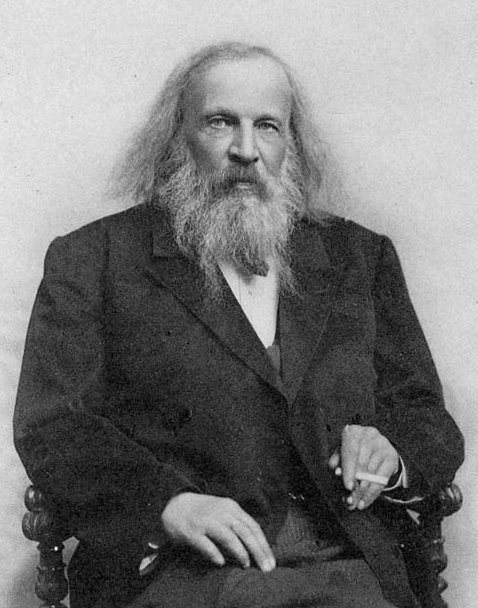
\includegraphics[width=\linewidth]{images/book1/mendeleev.jpg}

{\small ديمتري مندلييف (1834--1907).}
\end{minipage}\hfill
\begin{minipage}[b]{0.6\linewidth}\centering
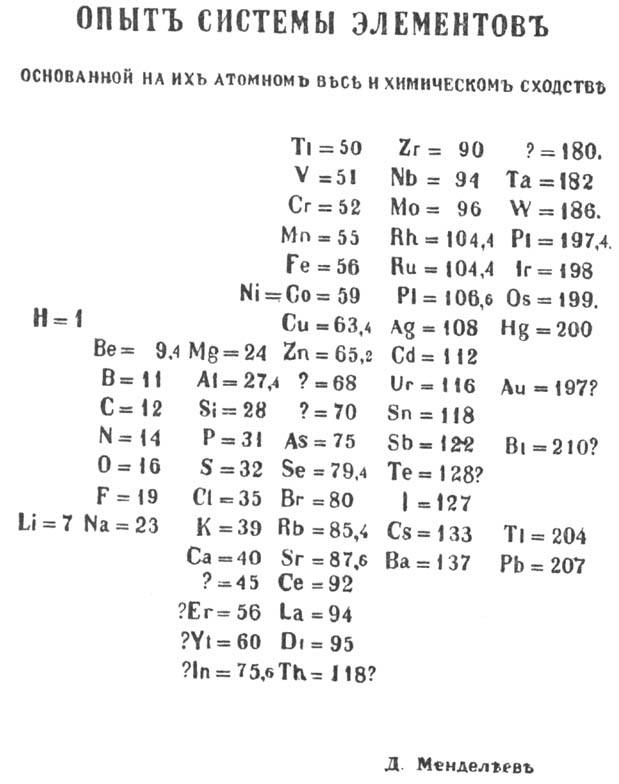
\includegraphics[width=0.85\linewidth]{images/book1/mendeleev-1869.jpg}

{\small جدول مندلييف لسنة 1869، بالروسية. بجوار Si $= 28$
وAl $= 27.4$ تنتظر الفجوتان «? $= 70$» و«? $= 68$» الجرمانيوم
والغاليوم.}
\end{minipage}
\end{omfigure}

\begin{remark}[الترتيب بحسب العدد الذري]\label{rem:g9:periodic-table-first-look:order}
رتّب مندلييف العناصر بحسب الوزن الذري، واضطر إلى مبادلة بضعة أزواج، مثل
التيلوريوم واليود، ليُبقي العائلات متجمعة. أما اليوم فيُرتَّب الجدول بحسب \omterm{def:g9:inside-the-atom:atomic-number}{العدد
الذري}، الذي اكتُشف لاحقًا، فلم تعد تلك المبادلات
لازمة.
\end{remark}

\section{تمارين}

\begin{exercise}[$\star$]\label{exo:g9:periodic-table-first-look:1}
بأي ترتيب توضع العناصر في \omterm{def:g9:periodic-table-first-look:periodic-table}{الجدول الدوري}؟
\end{exercise}

\begin{exercise}[$\star$]\label{exo:g9:periodic-table-first-look:2}
أعطِ \omterm{def:g9:periodic-table-first-look:period}{الدورة} \omterm{def:g9:periodic-table-first-look:period}{والزمرة} لكل من: الكربون ($Z = 6$)، والمغنيسيوم ($Z = 12$)،
والأرغون ($Z = 18$).
\end{exercise}

\begin{exercise}[$\star$]\label{exo:g9:periodic-table-first-look:3}
\omterm{def:g9:periodic-table-first-look:metal}{فلز} أم \omterm{def:g9:periodic-table-first-look:metal}{لافلز}: الحديد، والكبريت، والنحاس، والأكسجين، والألومنيوم، والكلور؟
\end{exercise}

\begin{exercise}[$\star$]\label{exo:g9:periodic-table-first-look:4}
أي عنصر يقع مباشرة تحت الصوديوم في الجدول؟ وأي عنصر مباشرة تحت الكلور؟
\end{exercise}

\begin{exercise}[$\star\star$]\label{exo:g9:periodic-table-first-look:5}
مستعينًا بالجدول، سمِّ عنصر \omterm{def:g9:periodic-table-first-look:period}{الدورة} 4 \omterm{def:g9:periodic-table-first-look:period}{والزمرة} 2، وعنصر \omterm{def:g9:periodic-table-first-look:period}{الدورة} 2
\omterm{def:g9:periodic-table-first-look:period}{والزمرة} 15.
\end{exercise}

\begin{exercise}[$\star\star$]\label{exo:g9:periodic-table-first-look:6}
لماذا نتوقع أن يتفاعل البوتاسيوم مع الماء كما يتفاعل الصوديوم؟
\end{exercise}

\begin{exercise}[$\star\star$]\label{exo:g9:periodic-table-first-look:7}
عنصر لامع يوصل الكهرباء ويكوّن \omterm{def:g9:ions:ion}{الأيون} \ce{X^{2+}}. هل هو \omterm{def:g9:periodic-table-first-look:metal}{فلز} أم
\omterm{def:g9:periodic-table-first-look:metal}{لافلز}؟ علّل.
\end{exercise}

\begin{exercise}[$\star\star$]\label{exo:g9:periodic-table-first-look:8}
لماذا ترك مندلييف فجوات في جدوله؟ ولماذا كان ذلك نقطة قوة في جدوله لا نقطة
ضعف؟
\end{exercise}

\begin{exercise}[$\star\star$]\label{exo:g9:periodic-table-first-look:9}
انظر إلى جدول مندلييف لسنة 1869. أي وزنين ذريين أعطى للكربون وللأكسجين؟
وأي فجوتين، معلَّمتين بعلامة استفهام، تظهران بجوار الألومنيوم
والسيليكون؟
\end{exercise}

\begin{exercise}[$\star\star$]\label{exo:g9:periodic-table-first-look:10}
كم عنصرًا في \omterm{def:g9:periodic-table-first-look:period}{الدورة} 2؟ وفي \omterm{def:g9:periodic-table-first-look:period}{الدورة} 4؟
\end{exercise}

\begin{exercise}[$\star\star\star$]\label{exo:g9:periodic-table-first-look:11}
الهيليوم والنيون والأرغون لا تكاد تتفاعل مع أي شيء. في أي \omterm{def:g9:periodic-table-first-look:period}{زمرة} هي؟ وفيمَ
يمكن أن تُستعمل، بالنظر إلى هذه الخاصية؟
\end{exercise}

\begin{exercise}[$\star\star\star$]\label{exo:g9:periodic-table-first-look:12}
اكتُشف الغاليوم، الذي يقع تحت الألومنيوم، سنة 1875. وكان مندلييف قد تنبأ له
بوزن ذري قريب من متوسط جاريه الألومنيوم (27.0) والإنديوم (114.8). احسب
هذا المتوسط. (الغاليوم: 69.7.)
\end{exercise}

\section{مسألة: فجوة مندلييف}

\begin{problem}[{مسألة نهاية الأسبوع --- التنبؤ بالوزن الذري لعنصر
مفقود انطلاقًا من جيرانه الأربعة}]
\label{pb:g9:periodic-table-first-look:1}
% ledger: aw:Si, aw:Sn, aw:Ga, aw:As, aw:Ge, mend:eka-si-aw, ge:winkler-aw
تنبأ مندلييف سنة 1871 بخصائص «إيكا سيليكون»، العنصر المفقود تحت السيليكون.
وكانت إحدى أفكاره أن خصائص العنصر تقع بين خصائص جيرانه فوقه وتحته، وعن
يساره وعن يمينه. والأوزان الذرية الحالية لجيران الفجوة الأربعة هي:
السيليكون 28.1 (فوقها)، والقصدير 118.7 (تحتها)، والغاليوم 69.7 (عن
يسارها)، والزرنيخ 74.9 (عن يمينها).

\medskip
\noindent\textbf{الجزء الأول --- الفجوة.}
\begin{enumerate}
  \item مستعينًا \omterm{def:g9:periodic-table-first-look:periodic-table}{بالجدول الدوري} في هذا الفصل، جد \omterm{def:g9:inside-the-atom:atomic-number}{العدد الذري} للجرمانيوم،
        العنصر الذي يملأ الفجوة، ودورته
        وزمرته.
  \item أي عنصر فوقه، وأيها تحته، وأيها عن يساره، وأيها عن
        يمينه؟
  \item هل الجرمانيوم \omterm{def:g9:periodic-table-first-look:metal}{فلز} أم \omterm{def:g9:periodic-table-first-look:metal}{لافلز} أم شبه \omterm{def:g9:periodic-table-first-look:metal}{فلز}؟
  \item لماذا توقع مندلييف أن يشبه العنصر المفقود
        السيليكون؟
\end{enumerate}

\medskip
\noindent\textbf{الجزء الثاني --- المتوسطات.}
\begin{enumerate}[resume]
  \item احسب متوسط الوزنين الذريين للعنصرين الواقعين فوق الفجوة
        وتحتها.
  \item احسب متوسط الوزنين الذريين للعنصرين الواقعين عن يسارها وعن
        يمينها.
  \item أي المتوسطين أقرب إلى الوزن الذري الحقيقي للجرمانيوم، 72.6؟ ولماذا
        قد يكون ذلك؟
  \item في جدوله لسنة 1869 كتب مندلييف «? $= 70$» لهذه
        الفجوة. بكم أخطأ؟
\end{enumerate}

\medskip
\noindent\textbf{الجزء الثالث --- التنبؤ.}
\begin{enumerate}[resume]
  \item احسب متوسط الجيران الأربعة جميعًا، بمنزلة عشرية
        واحدة.
  \item تنبأ مندلييف سنة 1871 بالقيمة 72؛ وقاس فينكلر سنة 1886 القيمة 72.3.
        قارنهما بمتوسطك.
  \item لماذا أقنع اكتشاف الجرمانيوم كثيرًا من الكيميائيين بصحة جدول
        مندلييف؟
  \item اذكر تنبؤك: الوزن الذري لإيكا سيليكون انطلاقًا من متوسط جيرانه
        الأربعة.
\end{enumerate}
\end{problem}
